% 代码测试
\section{算法测试效率}
\subsection{正常使用测试}
首先启动FlightAgent,然后启动Alice,可以看到Alice可以与FlightAgent正确协商密钥并进行合作订购机票,效果如下图:
\begin{figure}[H]
    \centering
    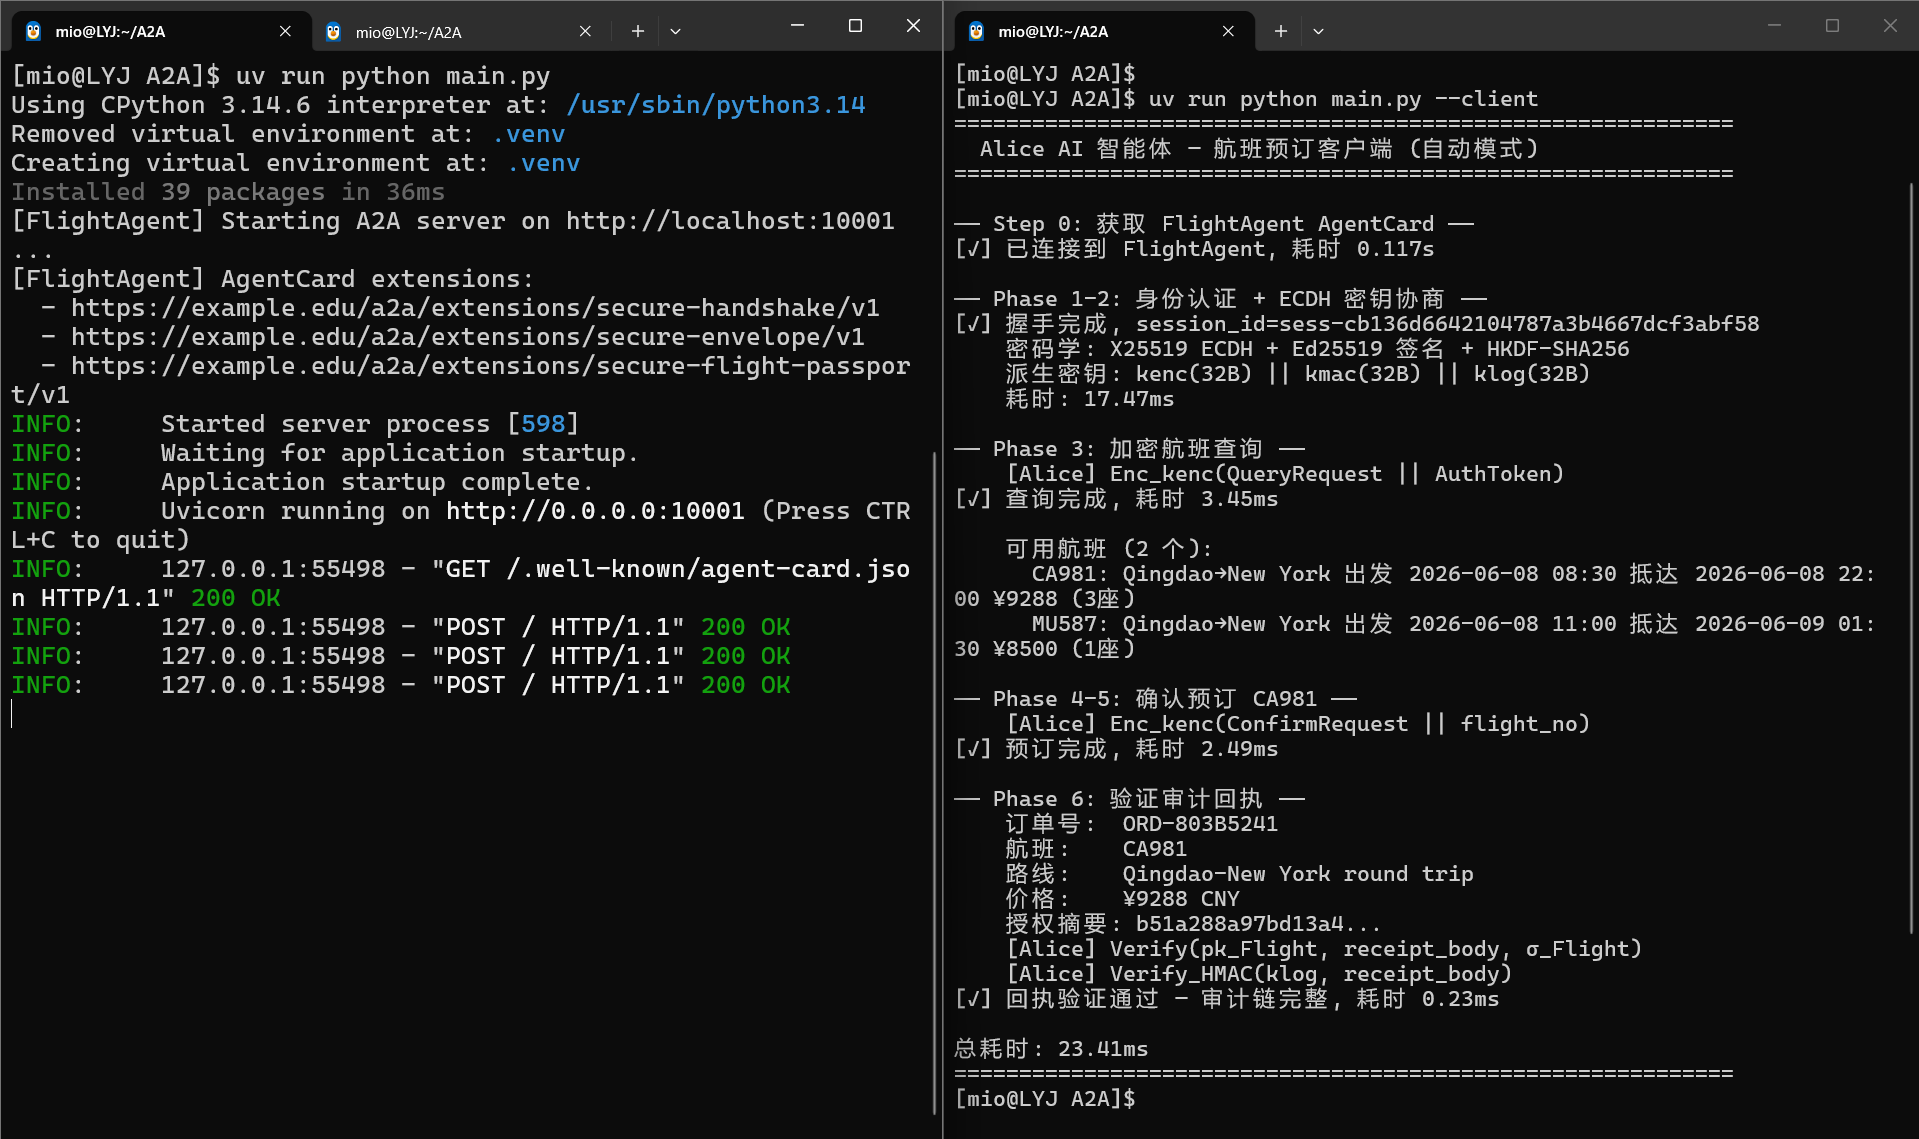
\includegraphics[width = 0.75\textwidth]{figures/normal_run.png}
    \caption{正常使用测试}
\end{figure}
整体耗时23.41ms,其中各个阶段耗时由上可得下表:

\begin{table}[H]
    \centering
    \caption{正常流程各阶段性能数据}
    \begin{tabular}{@{}llcc@{}}
        \toprule
        阶段 & 描述 & 耗时 & 占比 \\
        \midrule
        Step 0   & 获取 FlightAgent AgentCard（证书获取与连接） & $117.00$\,ms  & 99.5\% \\
        Phase 1--2 & 身份验证 + ECDH 密钥协商（X25519+HKDF） & $17.47$\,ms  & 74.6\% \\
        Phase 3   & 加密航班查询（AES-GCM封装/解封）           & $3.44$\,ms   & 14.7\% \\
        Phase 4--5 & 确认预订（签名回执生成）                 & $2.49$\,ms   & 10.6\% \\
        Phase 6   & 审计回执验证（Ed25519验签+HMAC）          & $0.25$\,ms   & 1.1\% \\
        \midrule
        \textbf{总计} & —                                    & $\mathbf{23.41}$\,\textbf{ms} & — \\
        \bottomrule
    \end{tabular}
\end{table}

\subsection{异常测试}
\begin{itemize}
    \item 重放攻击测试:截取历史合法消息，重复发送,结果如下图:
    \begin{figure}[H]
        \centering
        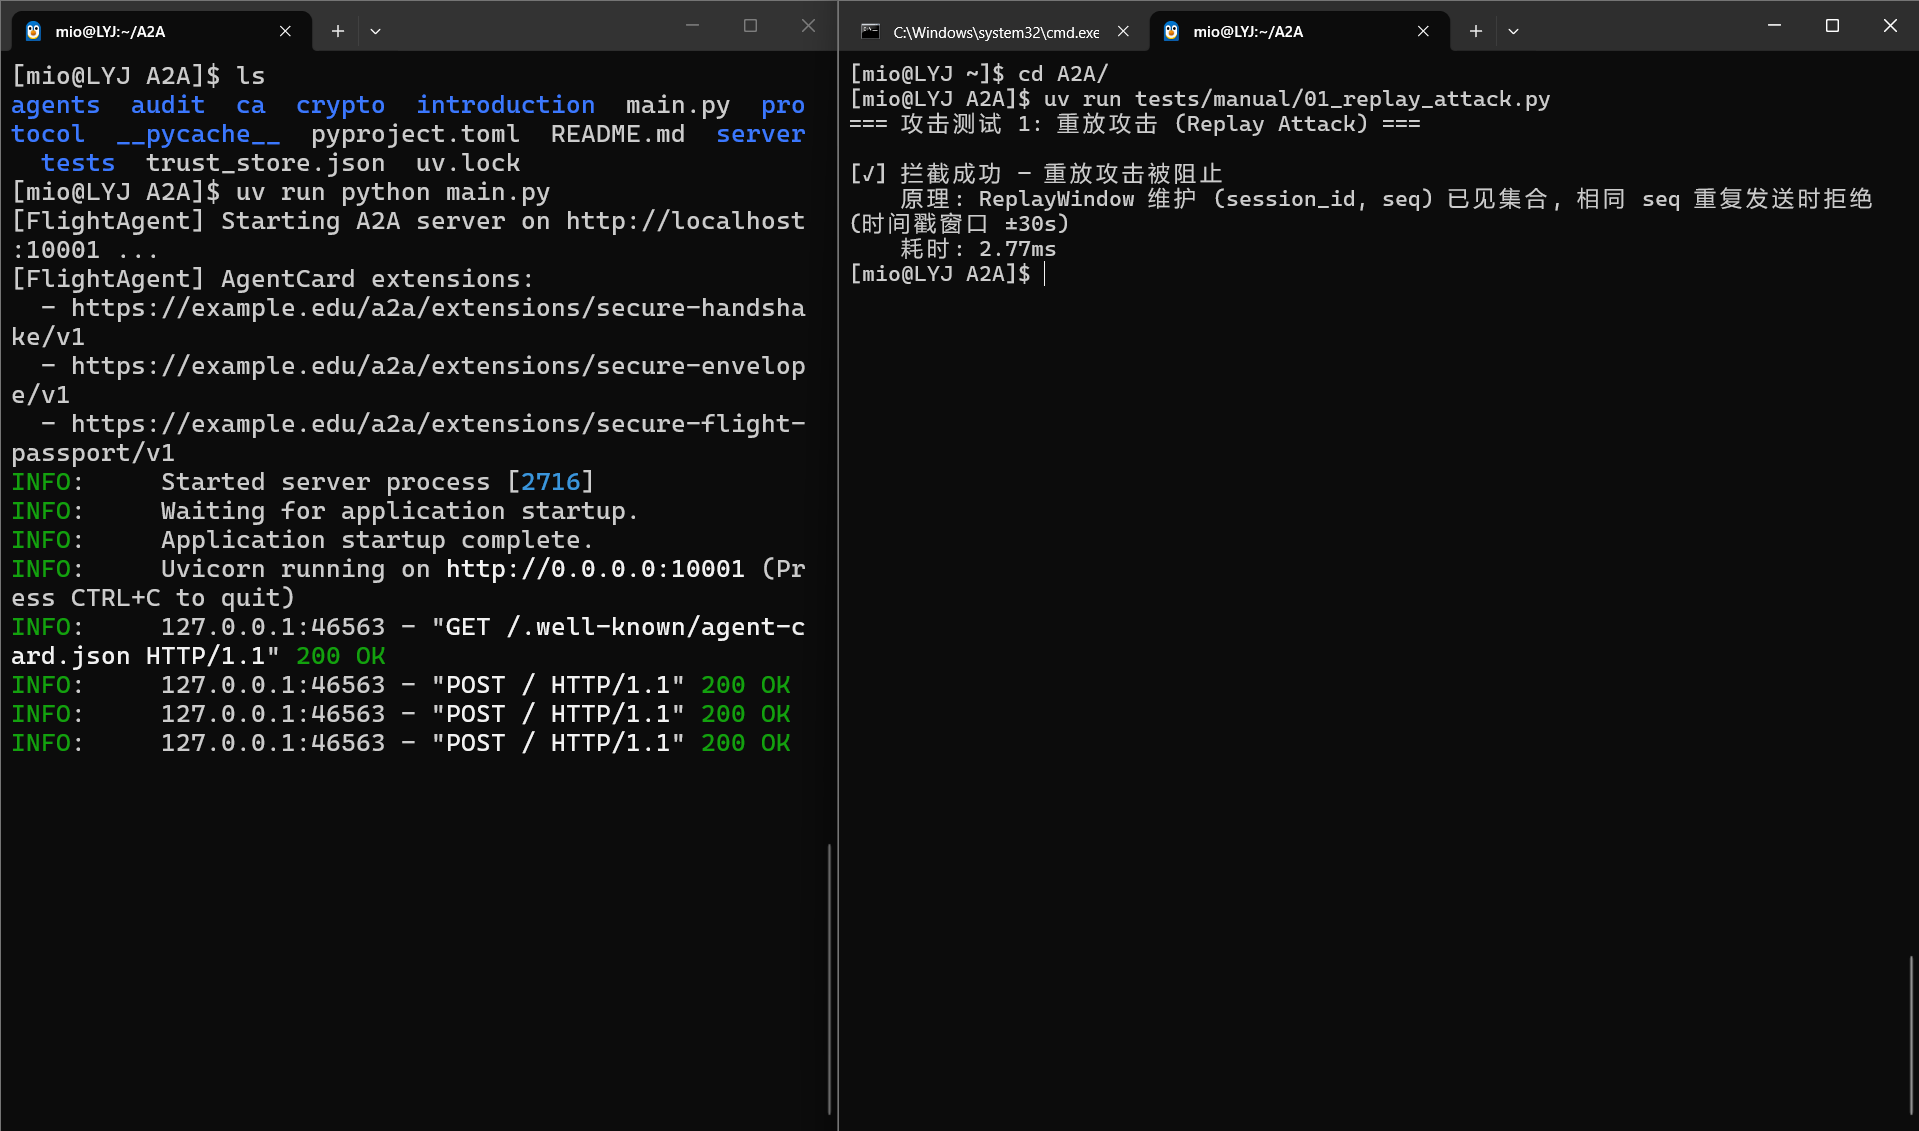
\includegraphics[width = 1\textwidth]{figures/replay.png}
        \caption{重放攻击测试}
    \end{figure}
    \item 授权扩权测试:手动篡改授权凭证预算金额，验证签名校验是否拦截篡改
请求,禁止扩权(这里将预算手动改为50000,权限手动添加一个"admin.delete_all"字段):
    \begin{figure}[H]
        \centering
        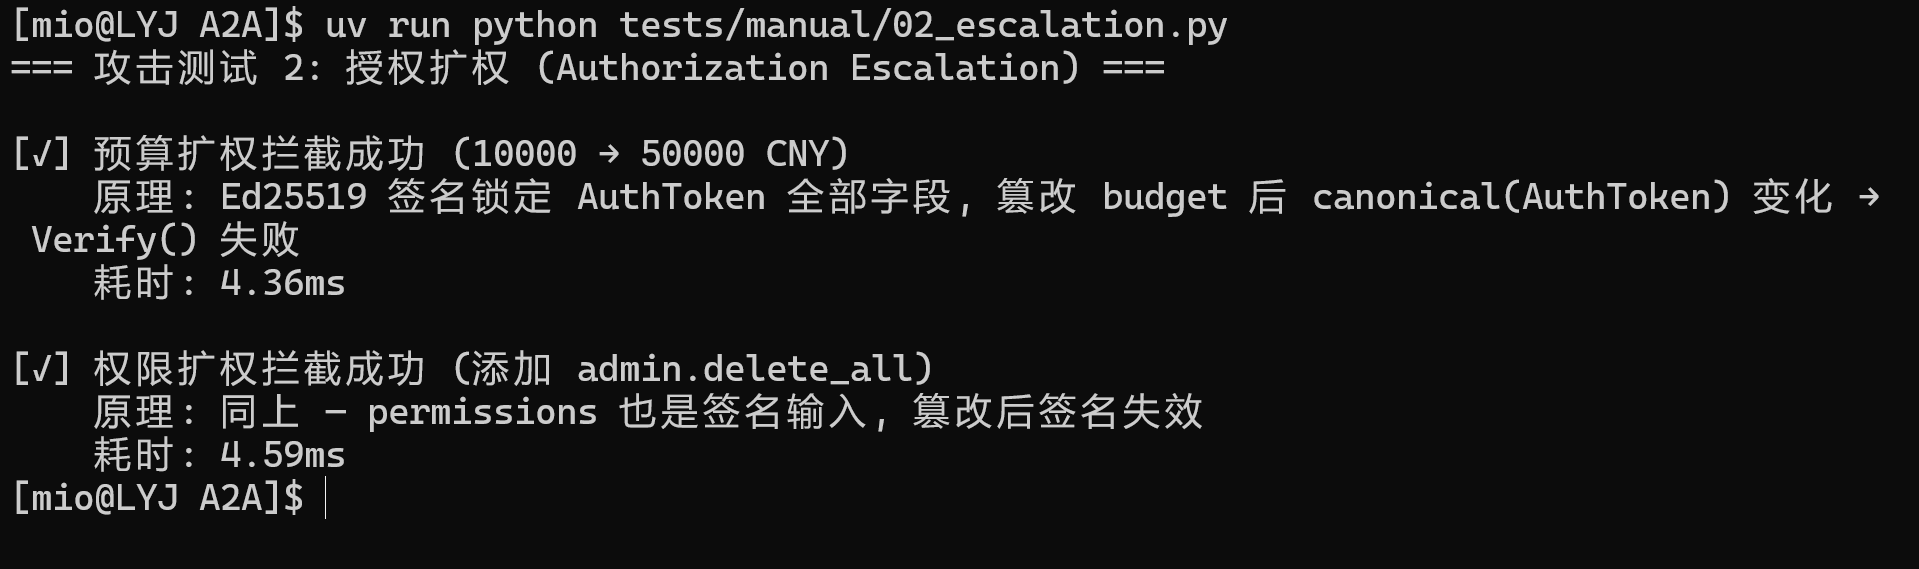
\includegraphics[width = 1\textwidth]{figures/budget_permission_modify.png}
        \caption{授权扩权测试}
    \end{figure}
    \item 消息篡改测试：修改传输中的订单价格、行程信息，验证 HMAC 完整性校验
是否识别篡改:
    \begin{figure}[H]
        \centering
        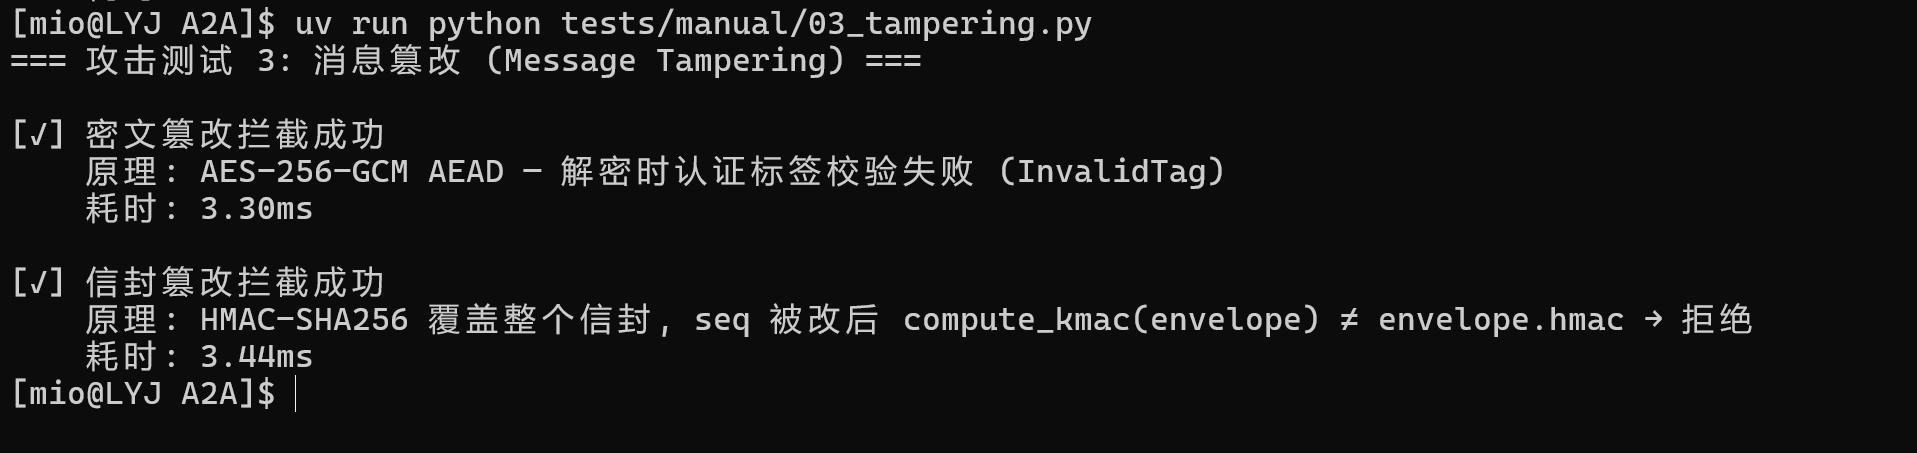
\includegraphics[width = 1\textwidth]{figures/message_modify.png}
        \caption{消息篡改测试}
    \end{figure}
    \item 伪造身份测试：使用非法凭证、伪造智能体身份(这里使用非法第三方CA签发的证书)发起请求，验证身份绑定
机制是否拦截非法接入。
    \begin{figure}[H]
        \centering
        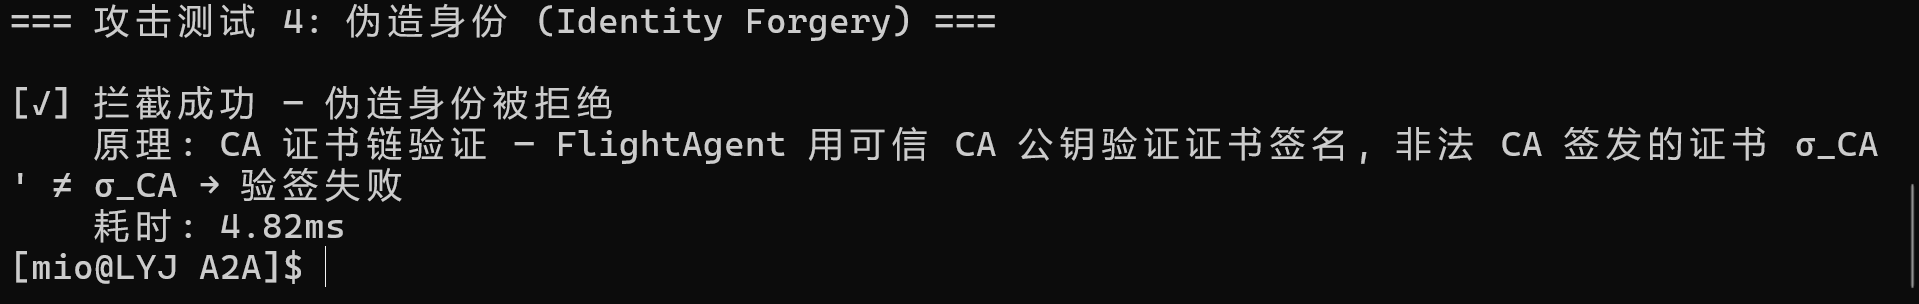
\includegraphics[width = 1\textwidth]{figures/illigal_agent.png}
        \caption{伪造身份测试}
    \end{figure}
\end{itemize}
综上该协议能正确检测出这些异常情况并及时响应,确保系统的安全性。测试异常检测数据总结如下表:

\begin{table}[H]
    \centering
    \caption{异常攻击检测结果汇总}
    \small
    \begin{tabularx}{\textwidth}{@{}llXc@{}}
        \toprule
        攻击类型 & 检测结果 & 防护机制 & 耗时 \\
        \midrule
        重放攻击 & 拦截成功 & ReplayWindow 维护 (session\_id, seq) 已见集合，相同 seq 重复发送时拒绝 & $2.77$\,ms \\
        预算扩权 & 拦截成功 & Ed25519 签名锁定 AuthToken 全部字段，篡改 budget 后 canonical() 变化导致 Verify() 失败 & $4.36$\,ms \\
        权限扩权 & 拦截成功 & 同上——permissions 也是签名输入，篡改后签名失效 & $4.59$\,ms \\
        密文篡改 & 拦截成功 & AES-256-GCM AEAD 解密时认证标签校验失败（InvalidTag）& $3.30$\,ms \\
        信封/序号篡改 & 拦截成功 & HMAC-SHA256 覆盖整个信封，seq 被改后 compute\_kmac $\neq$ envelope.hmac，拒绝 & $3.44$\,ms \\
        伪造身份 & 拦截成功 & CA 证书链验证：非法 CA 签发的证书 $\sigma_{CA}' \neq \sigma_{CA}$，验签失败 & $4.82$\,ms \\
        \bottomrule
    \end{tabularx}
\end{table}
